\begin{frame}{}
    \LARGE VAE: \textbf{Latent Variable Models}
\end{frame}

\begin{frame}[allowframebreaks]{Latent Variable Models}
\begin{itemize}
    \item \textbf{Autoregressive models + Flows}: All random variables are observed.
    \item \textbf{Latent Variable Models (LVMs)}: Some random variables are hidden -- we do not get to observe them.
\end{itemize}
\vspace{1em}
\begin{columns}
        \begin{column}{0.6\linewidth}
            \begin{figure}
                \centering
                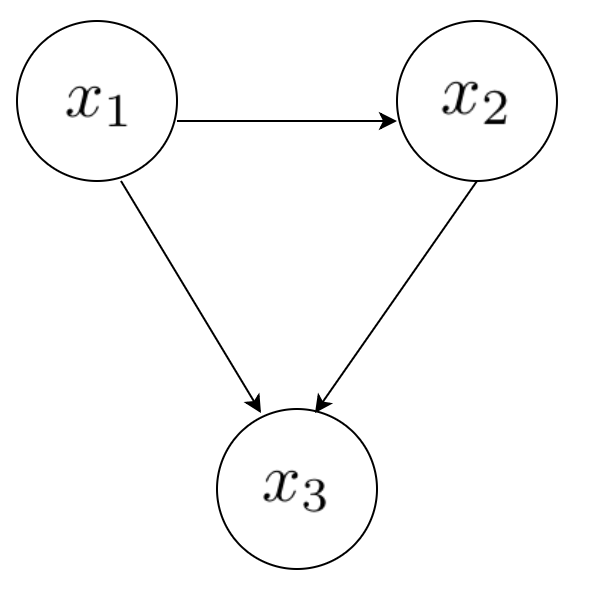
\includegraphics[height=0.6\textheight]{images/vae/latent-graph-1.png}
            \end{figure}
        \end{column}
        \begin{column}{0.4\linewidth}
            \begin{figure}
                \centering
                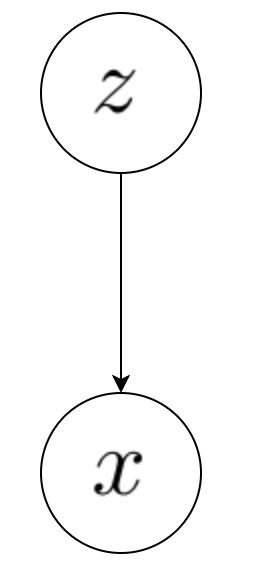
\includegraphics[height=0.6\textheight]{images/vae/latent-graph-2.png}
            \end{figure}
        \end{column}
    \end{columns}

\framebreak

\textbf{Latent Variable Models}:
\begin{itemize}
    \item \textbf{Definition}: Models that assume the data is generated from some unobserved (latent) variables.
    \item \textbf{Goal}: Learn a mapping from observed data \( x \) to latent variables \( z \) and vice versa.
    \item \textbf{Generative Process}:
        \begin{itemize}
            \item Sample latent variable \( z \) from a prior distribution \( p(z) \).
            \item Generate data \( x \) from the latent variable using a likelihood function \( p(x|z) \).
        \end{itemize}
    \item \textbf{Inference Problem}: Given observed data \( x \), infer the posterior distribution \( p(z|x) \).
    \item \textbf{Challenge}: Direct computation of posterior \( p(z|x) \) is often intractable, leading to the need for approximations.
\end{itemize}
\end{frame}

\begin{frame}[allowframebreaks]{Why Latent Variable Models?}
    \begin{itemize}
        \item Simpler, lower-dimensional representations of data often possible
        \begin{itemize}
            \item Latent variable models hold the promise of automatically identifying those hidden representations
        \end{itemize}
    \end{itemize}
    \begin{figure}
        \centering
        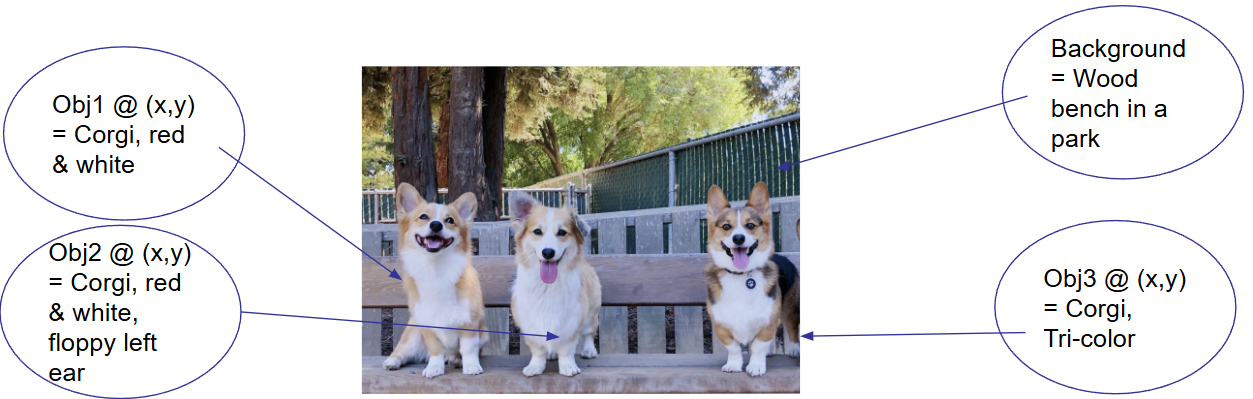
\includegraphics[height=0.5\textheight]{images/vae/why-latent.png}
    \end{figure}

    \framebreak

    \begin{itemize}
        \item Autoregressive (AR) models are slow to sample because all pixels (observation dimensions) are assumed to be dependent on each other.
        \item We can make part of the observation space independent \textit{conditioned on some latent variables}.
        \item Latent variable models \textit{can} have faster sampling by exploiting statistical patterns.
    \end{itemize}

    \framebreak

    \begin{itemize}
        \item Sometimes, it’s possible to design a latent variable model with an understanding of the causal process that generates data
        \item In general, we don’t know what are the latent variables and how they interact with observations
        \item Most popular models make little assumption about what are the latent variables
        \item Best way to specify latent variables is still an active area of research
    \end{itemize}
\end{frame}

\begin{frame}[allowframebreaks]{Latent Variable Model}
    \begin{figure}
        \centering
        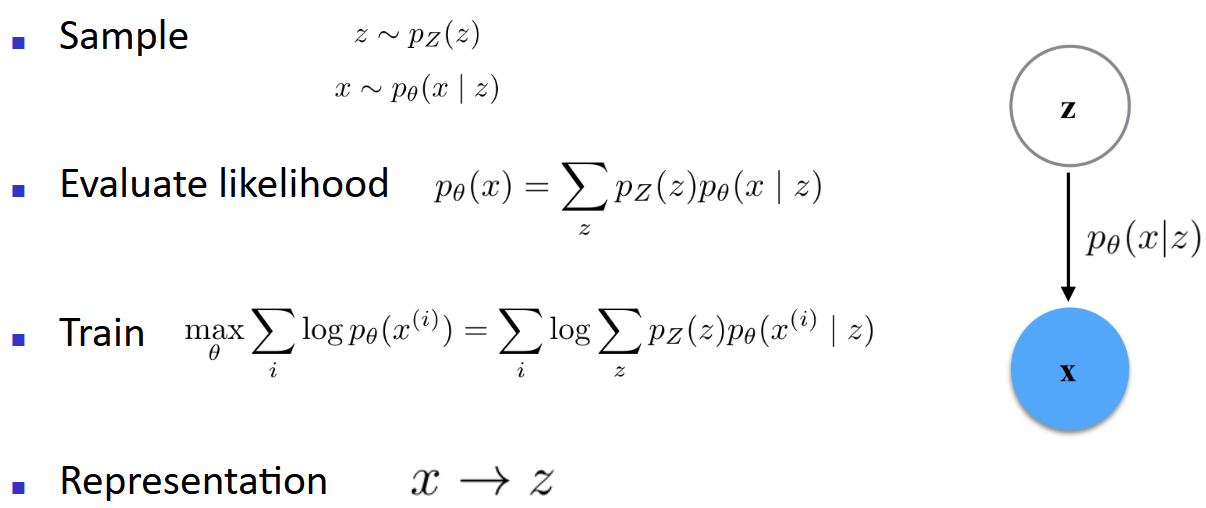
\includegraphics[width=\linewidth]{images/vae/latent-variable-model.png}
    \end{figure}
\end{frame}
